
\section{Appendix}\label{sec:appendix}


\subsection{Gaussian-sigmoid function}
\noindent The function $\Phi_{\cdot}$ is defined by combining a generalized version of the sigmoid, namely with a gain $\beta \neq 1$ and offset $\alpha\neq 0$, and a Gaussian with mean $\mu$ and variance $\sigma$. Their contributions are weighted by as $r$ and $1-r$ ($r\in(0,1)$) respectively.

\begin{equation*}
    \Phi_v(x) = r\left(1 + \exp^{-\beta(x-\alpha)}\right)^{-1} + (1-r)\exp\left(-\frac{(x-\mu)^2}{2\sigma^2}\right)
\end{equation*}

\noindent The motivation behind this choice is to express a function that possesses a bounded region (depending on $\mu,\,\sigma$) at a high/low peak (depeding on the value of $\gamma_{2}$), and a continuous transition to a constant value (depending on the steepness of the sigmoid $\beta$, shift
$\alpha$, and intensity $\gamma_{1}$).

\begin{figure}[ht]
    \centering
    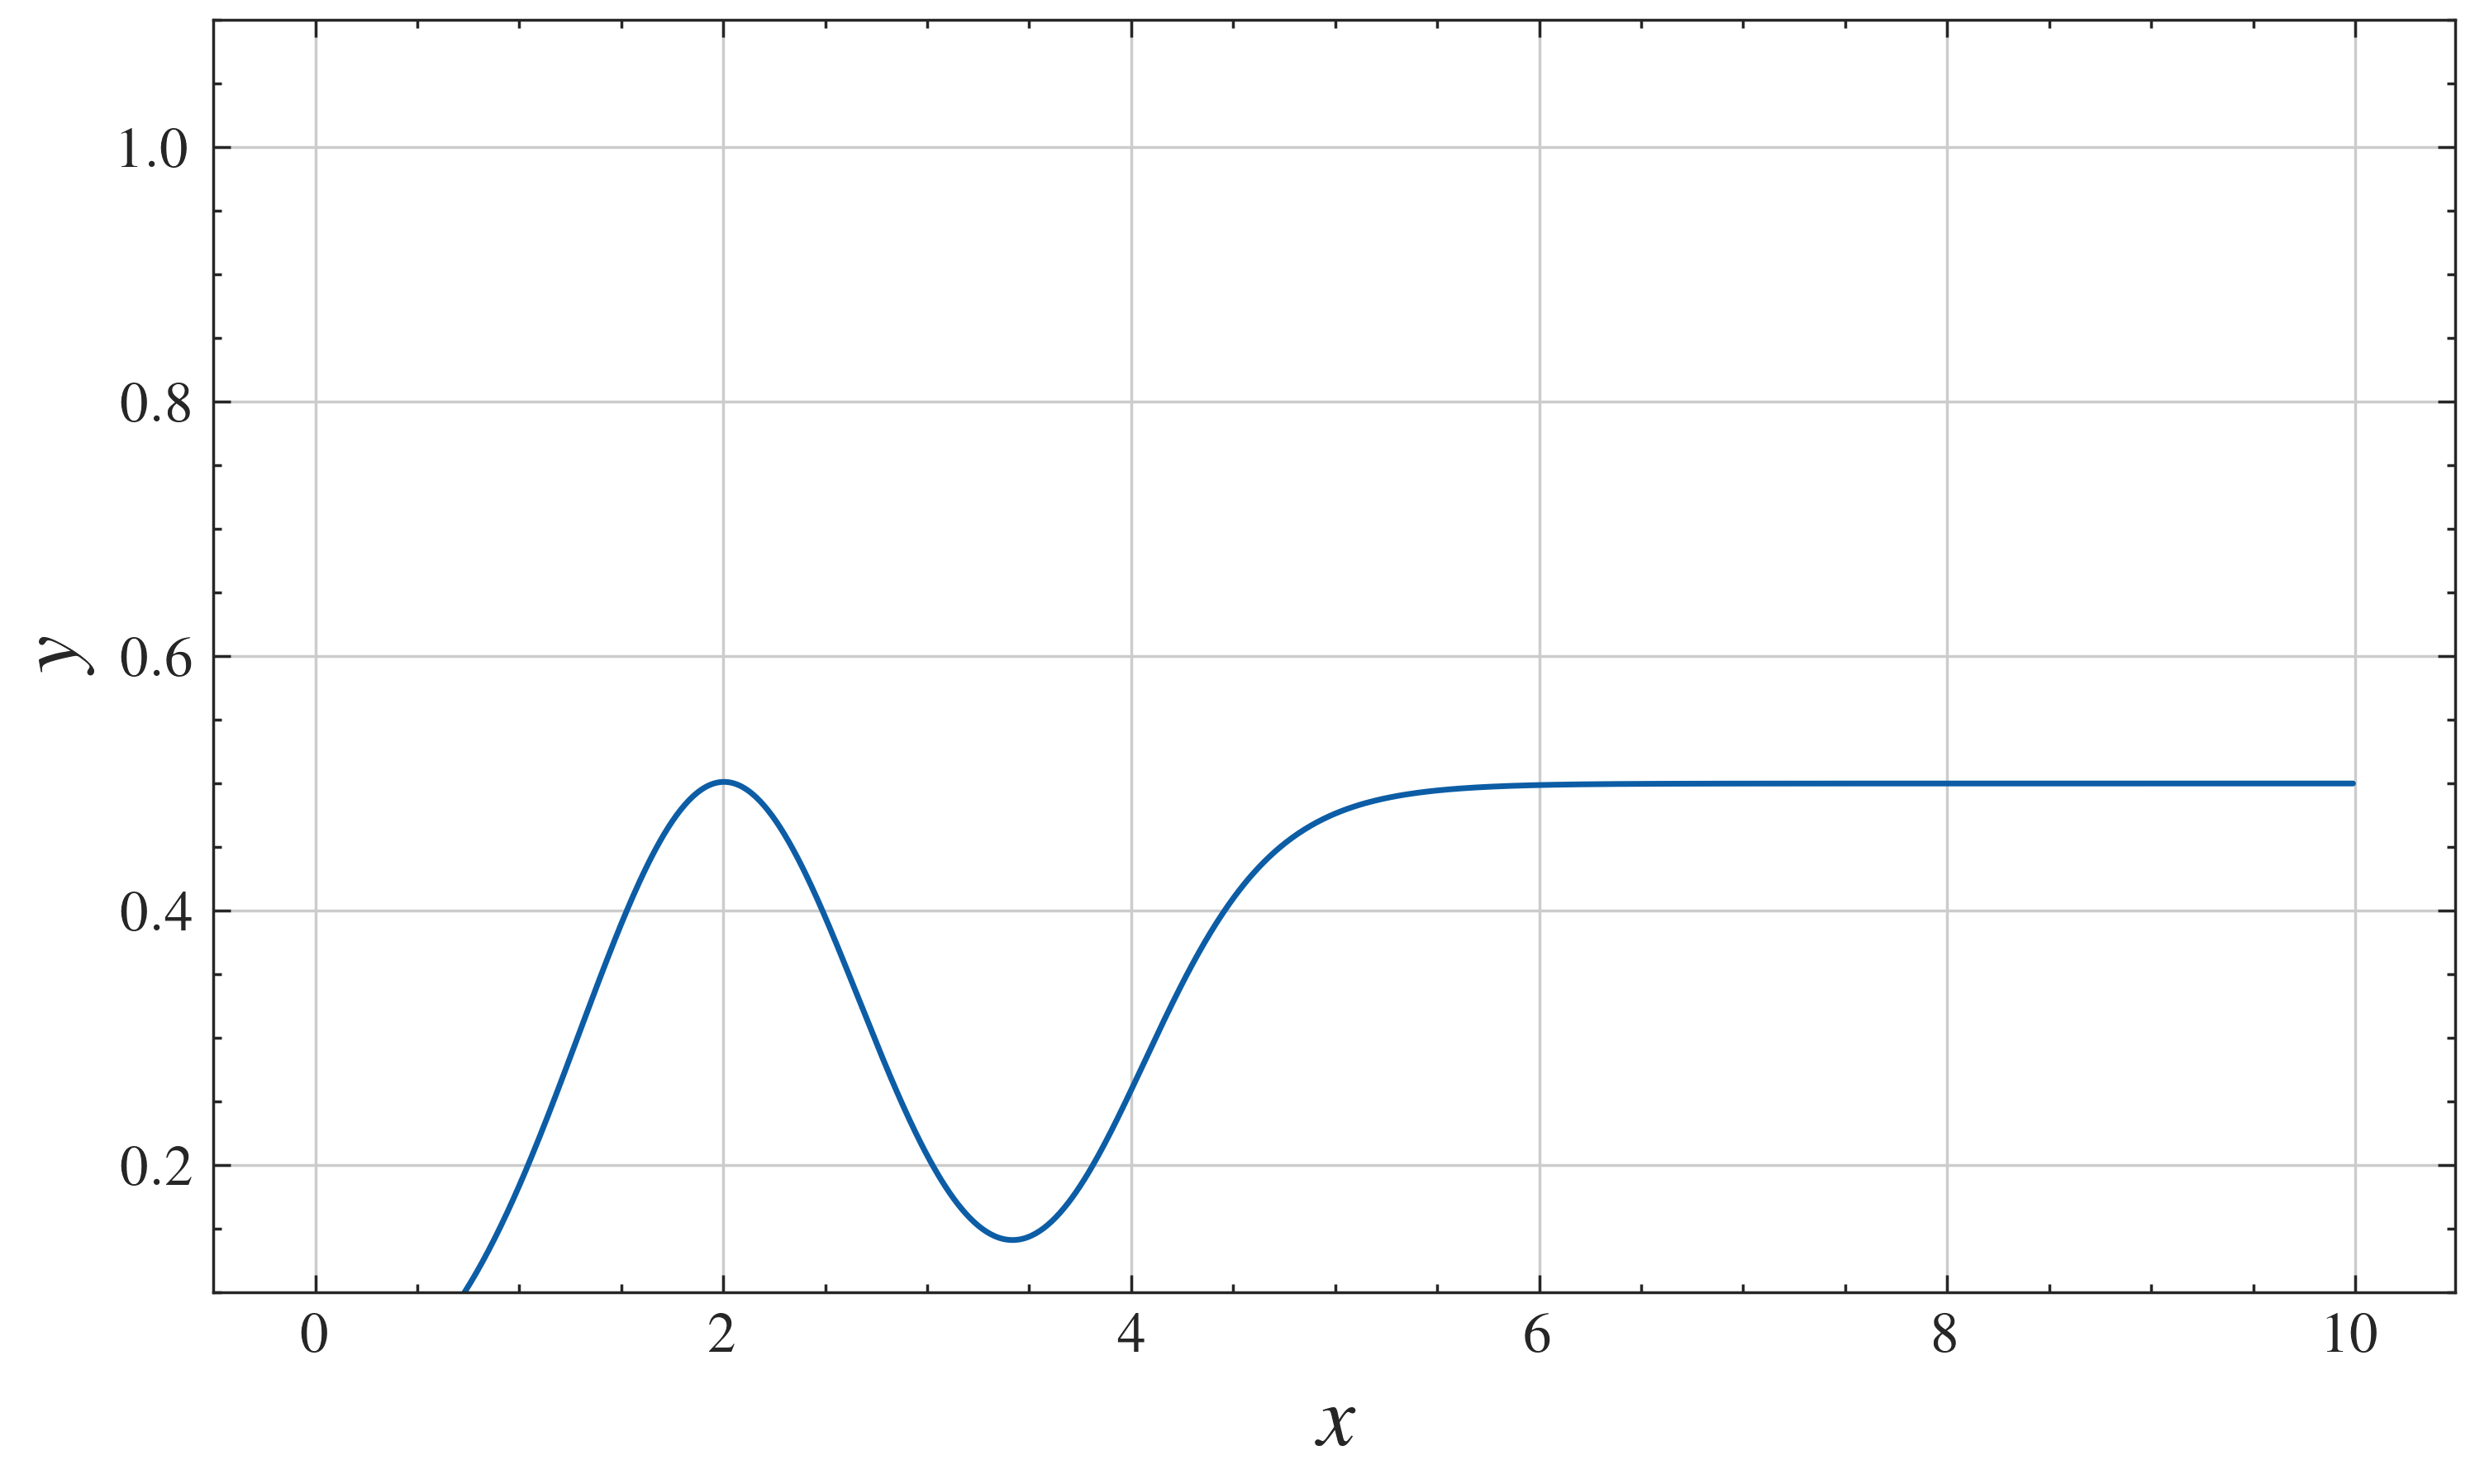
\includegraphics[width=0.8\textwidth]{figures/gaussian_sigmoid.png}
    \caption{\textsc{Activation function $\Phi_{v}$} - \textit{Parameters $\beta=10$, $\alpha=1$, $\mu=1$, $\sigma=1$, and $r=0.5$.}}
    \label{fig:gau_sigm}
\end{figure}


\subsection{Evolution search stup}
The optimization was carried out over several parameters concerning the model architecture and dynamics:
\textbf{Network parameters}
\begin{itemize}
    \item $\tau_{u}$: time constant of population $u$ ($M$)
    \item $\tau_{v}$: time constant of population $v$ ($V$)
    \item $g$: gain of the sigmoidal activation function of population v
    \item $\theta$: threshold of the sigmoidal activation function of population v
    \item $W^{+}$: maximal weight value for the weights $\textbf{W}^{MV}$
\end{itemize}

\noindent \textbf{Option value function parameters}
\begin{itemize}
    \item $\beta_{v}$: steepness of the sigmoid
    \item $\alpha_{v}$: shift of the sigmoid
    \item $\mu_{v}$: mean of the Gaussian
    \item $\sigma_{v}$: variance of the Gaussian
    \item $r_{v}$: weight of the sigmoid
\end{itemize}

\noindent \textbf{Learning rate function parameters}
\begin{itemize}
    \item $\gamma_{\eta}$: intensity of the l
    \item $\beta_{\eta}$: steepness of the sigmoid
    \item $\alpha_{\eta}$: shift of the sigmoid
    \item $\mu_{\eta}$: mean of the Gaussian
    \item $\sigma_{\eta}$: variance of the Gaussian
    \item $r_{\eta}$: weight of the sigmoid
\end{itemize}

\noindent Each individual has been evaluated over environment the following environments:

\begin{itemize}
    \item \textsc{MAB-0}: average reward distribution entropy $\langle H\rangle=2.05$
    \item \textsc{KAB-$\sin$P}: average reward distribution entropy $\langle H\rangle=2.1$, given $K$ arm frequencies as an equally spaced set $\{0.1\ldots i\ldots 0.4\}$, phases drawn from an uniform $\sim \mathcal{U}(0, 2\pi)$, and half of the arms have been set to constant values drawn from
        another uniform $\sim \mathcal{U}(0.1, 0.7)$; the final reward distribution was not normalized.
\end{itemize}

\noindent The number of arms was $K=10$ and $150$, and lasted for $2$ trials with $2000$ rounds each.
The final fitenss was the average over $2$ iterations.

\hfill \break
The optimization has been implemented in Python using the \texttt{DEAP} library, and the algorithm used was the \texttt{CMA-es} algorithm. The optimization involved $70$ generations with a population size of $128$ individuals. The mutation rate was set to $0.5$ with a sigma of $0.8$, the cross-over rate was set to $0.4$.
The run were carried out on a 256-core AMD EPYC 7763 with 2TB of RAM.


\subsection{Reward distribution entropy}\label{sec:appendix_entropy}

\noindent The calculation of a set of $N$ reward probability distribution $\mathbf{p}_{i}\text{  for  } i\ldots N$ for $K$ values with a progressively decreasing levels of entropy $\mathbf{h}_{i}\text{  for  } i\ldots N$ has been obtained by the following algorithm:

\begin{algorithm}[ht]
\caption{Reward Probability Distribution Generation}
\label{alg:reward_distribution}
\SetAlgoLined
\KwIn{Number of distributions $N$, dimension $K$}
\KwOut{Set of probability distributions ${\mathbf{p}_i}$ with decreasing entropy}
\SetKwComment{Comment}{// }{ }
\textbf{Initial Setup:}
Define set $B = \{1.5^x \mid x = 1, \ldots, 7\}$; \\
\For{$i \gets 1$ to $N$}{
$\mathbf{z} \gets \text{RandomVector}(0,1)^K$;\\
$j \gets \text{RandomIndex}(K)$;\\
$\mathbf{z}_j \gets 1$;\\
$\beta_i \gets \text{Sample index=} i \text{ from }(B)$ \Comment*[r]{Sample temperature from $B$}

$\mathbf{p}_i \gets \frac{\exp(\beta_i \mathbf{z})}{\sum_j \exp(\beta_i \mathbf{z}_j)}$ \Comment*[r]{Softmax with temperature}
}
\Return ${\mathbf{p}_i}$
\end{algorithm}


\subsection{Table of results}

% --- table K.5
\begin{table}[H]
\centering
\caption{Performance comparison for $K=5$}
\label{tab:k5}
\begin{tabular}{l c c c}
\toprule
\textbf{Model} & \textbf{\textsc{KAB-0}} & \textbf{\textsc{KAB-$\epsilon$}} & \textbf{\textsc{KAB-$\sin$}}\\
\midrule
Optimal & $0.900$ & $0.881$ & $0.563$ \\
Random & $0.330$ & $0.337$ & $0.200$ \\
\midrule
Thompson & $0.905$ & $0.617$ & $0.317$ \\
$\epsilon$-Greedy & $0.797$ & $0.531$ & $0.315$ \\
UCB & $0.897$ & $0.656$ & $0.319$ \\
\textbf{Model} & $\mathbf{0.899}$ & $\mathbf{0.663}$ & $\mathbf{0.265}$ \\

\bottomrule
\end{tabular}
\end{table}

% --- table K.10
\begin{table}[H]
\centering
\caption{Performance comparison for $K=10$}
\label{tab:k10}
\begin{tabular}{l c c c}
\toprule
\textbf{Model} & \textbf{\textsc{KAB-0}} & \textbf{\textsc{KAB-$\epsilon$}} & \textbf{\textsc{KAB-$\sin$}} \\
\midrule
Optimal & $0.900$ & $0.885$ & $0.355$  \\
Random & $0.247$ & $0.250$ & $0.100$ \\
\midrule
Thompson & $0.896$ & $0.648$ & $0.339$ \\

$\epsilon$-Greedy & $0.611$ & $0.597$ & $0.343$ \\
UCB & $0.891$ & $0.655$ & $0.358$ \\
\textbf{Model} & $\mathbf{0.905}$ & $\mathbf{0.668}$ & $\mathbf{0.203}$  \\
\bottomrule
\end{tabular}
\end{table}

% --- table K.100
\begin{table}[H]
\centering
\caption{Performance comparison for $K=100$}
\label{tab:k100}
\begin{tabular}{l c c c}
\toprule
\textbf{Model} & \textbf{\textsc{KAB-0}} & \textbf{\textsc{KAB-$\epsilon$}} & \textbf{\textsc{KAB-$\sin$}} \\
\midrule
Optimal & $0.900$ & $0.883$ & $0.020$  \\
Random & $0.196$ & $0.201$ & $0.010$ \\
\midrule
Thompson & $0.894$ & $0.586$ & $0.013$ \\
$\epsilon$-Greedy & $0.519$ & $0.574$ & $0.018$ \\
UCB & $0.853$ & $0.572$ & $0.012$ \\
\textbf{Model} & $\mathbf{0.898}$ & $\mathbf{0.651}$ & $\mathbf{0.010}$  \\
\bottomrule
\end{tabular}
\end{table}

% --- table K.200
\begin{table}[H]
\centering
\caption{Performance comparison for $K=100$}
\label{tab:k200}
\begin{tabular}{l c c c}
\toprule
\textbf{Model} & \textbf{\textsc{KAB-0}} & \textbf{\textsc{KAB-$\epsilon$}} & \textbf{\textsc{KAB-$\sin$}} \\
\midrule
Optimal & $0.900$ & $0.885$ & $0.010$  \\
Random & $0.178$ & $0.176$ & $0.005$ \\
\midrule
Thompson & $0.875$ & $0.624$ & $0.006$ \\
$\epsilon$-Greedy & $0.679$ & $0.588$ & $0.010$ \\
UCB & $0.792$ & $0.510$ & $0.006$ \\
\textbf{Model} & $\mathbf{0.905}$ & $\mathbf{0.610}$ & $\mathbf{0.006}$  \\
\bottomrule
\end{tabular}
\end{table}

% --- table K.1000
\begin{table}[H]
\centering
\caption{Performance comparison for $K=100$}
\label{tab:k1000}
\begin{tabular}{l c c c}
\toprule
\textbf{Model} & \textbf{\textsc{KAB-0}} & \textbf{\textsc{KAB-$\epsilon$}} & \textbf{\textsc{KAB-$\sin$}} \\
\midrule
Optimal & $0.900$ & $0.880$ & $0.002$  \\
Random & $0.177$ & $0.178$ & $0.001$ \\
\midrule
Thompson & $0.779$ & $0.445$ & $0.001$ \\
$\epsilon$-Greedy & $0.386$ & $0.478$ & $0.002$ \\
UCB & $0.301$ & $0.185$ & $0.001$ \\
\textbf{Model} & $\mathbf{0.703}$ & $\mathbf{0.480}$ & $\mathbf{0.001}$  \\
\bottomrule
\end{tabular}
\end{table}


\newpage
